\documentclass[12pt,a4paper]{article}

\usepackage{jyw-program}

\begin{document}
\title{期中考參考解答}
\author{Jia-Yin Wang}
\maketitle

\begin{abstract}
這份講義是這次甲乙班期中考的參考解答,主要是給同學做為學習參考之用。基本上學習程式,務求完全理解,最好還能實際上機測試,否則好像看過看懂,實際上在作答或應用的時候,還是沒有辦法弄出來。所以希望同學在閱讀的同時,可以多加思考,並且實際上機測試,以求完全了解。
\end{abstract}

\section{A009 - 質數判別}
輸入一個正整數,如果是質數,則輸出 Yes,如果不是,則輸出 No。

\subsection{解題思惟}
\begin{enumerate}
\item 質數的特色是除了1之外,另外一個唯一的因數就是n本身。所以從1檢查到n,應該有2個因數。以下的程式應該就可以判斷了。
	\begin{inside}
	int cnt=0;
	for (i=1; i<=n; i++) if (n%i==0) cnt++; // 檢查到因數,把個數加1。
	if (cnt==2) cout<<"Yes"; else cout<<"No";
	\end{inside}
\item 也可以只檢查2, …, n-1是否為n的因數,如果其中有一個因數,那n就不是質數了,否則n就是質數。在這種情況下,1和2應該要另外處理,1不是質數,但2是質數。
\item 可以設定一個旗標變數,如果沒有因數存在,把值設為1 (表示n為質數),當有任一個因數存在時,把它設為0 (表示n非質數)。預設值可以為1,檢查到因數時設為0。像以下這樣:
	\begin{inside}
	int flag=1;
	for (i=2; i<n; i++) if (n%i==0) { flag=0; break; }
	\end{inside}
\item 綜合2-3兩點,也可以用以下方式解此問題。
	\begin{inside}
	int flag=1; // 預設flag為1
	if (n==1) flag=0; // 1不是質數
	else if (n>3) { // 2和3是質數,flag不用變動,處理n>3情況即可
		for (i=2; i<n; i++) if (n%i==0) { flag=0; break; }
	}
	\end{inside}
\item  進階思考:實際上檢查$n$的因數只要檢查到$\sqrt{n}$即可,因為如果有個因數$x$超過$\sqrt{n}$,那麼$n/x$就小於$\sqrt{n}$,會先被檢查到。另外$i\le\sqrt{n}$可以改成$i*i\le n$。
\item 偶數不是質數,也可以先過濾掉,奇數的部份,只要檢查有沒有奇數的因數就可以了。
\end{enumerate}

\subsection{程式碼}
\begin{cppcode}
	#include <iostream>
	
	using namespace std;
	
	int main()
	{
		int i, n, flag=1;
		cin >> n;
		if (n==1) flag=0; // 1 非質數
		else if (n>3) { // 2和3是質數,flag不用變動,處理n>3情況即可
			if (n%2==0) flag=0; // 偶數非質數
			else for (i=3; i*i<=n; i+=2) { // 只檢查奇數i,範圍i*i<=n
				if (n%i==0) { flag=0; break; } // 發現因數,設定旗標跳出
			}
		}
		if (flag) cout << "Yes";
		else cout << "No";
		return 0;
	}
\end{cppcode}

\section{A020 - 韓信點兵}
韓信點兵, 7個一數剩3個, 9個一數剩4個, 10個一數剩2個, 11個一數剩1個, 請問韓信兵團至少有多少人?

\subsection{解題思惟}
\begin{enumerate}
	\item 因為要求最少可能的人數,所以可從1開始往上嘗試,當條件滿足時即可印出並離開迴圈。
	\item 在判斷條件時,可以使用 \&\& 把幾個條件串起來,全部符合時印出並跳出;或者個別測試,不符合時跳過。前者的用法如下:
	\begin{inside}
		if (i%7==3 && i%9==4 && i%10==2 && i%11==1) { ... }
	\end{inside}
	後者的用法如下:
	\begin{inside}
		if (i%7!=3) continue;
		if (i%9!=4) continue;
		if (i%10!=2) continue;
		if (i%11!=1) continue;
		...
	\end{inside}
\end{enumerate}


\subsection{程式碼}
\begin{cppcode}
	#include <iostream>
	
	using namespace std;
	
	int main() 
	{
		for (int i=1; ; i++) {
			if (i%7==3 && i%9==4 && i%10==2 && i%11==1) {
				cout << i;
				break;
			}
		}
		return 0;
	}
\end{cppcode}


\section{A025 - 判斷閏年}
輸入西元年,如果該年是閏年,則輸出Yes,若該年不是閏年,則輸出No。 (閏年的定義為,四年一閏,逢百不閏,逢四百又閏。例如西元1004年為閏年,西元1100年不是閏年,西元1600年是閏年)

\subsection{解題思維}
這一題可以使用巢狀的if-else依規則次序進行判斷,或者也可以使用複合的邏輯判斷式進行。方法有很多種,以下舉出三個方法供作參考。
\subsection{程式碼}
從400的倍數,100的倍數,4的倍數依次判斷
\begin{cppcode}
	#include <iostream>
	
	using namespace std;
	
	int main()
	{
		int year;
		cin >> year;
		if (year%400==0) cout << "Yes"; // 400的倍數
		else if (year%100==0) cout << "No"; // 否,但是100的倍數
		else if (year%4==0) cout << "Yes"; // 否,但是4的倍數
		else cout << "No";
		return 0;
	}
\end{cppcode}

\noindent 
從4的倍數,100的倍數,400的倍數依次判斷,這邊是判斷非其倍數為主。要判斷一數n不是k的倍數,可以寫 if (n\%k != 0),但是運算式不為0本來就代表true,所以也可以簡寫成 if (n\%k)。
\begin{cppcode}
	#include <iostream>
	
	using namespace std;
	
	int main()
	{
		int year;
		cin >> year;
		if (year%4) cout << "No"; // 不是4的倍數
		else if (year%100) cout << "Yes"; // 是,但不是100的倍數
		else if (year%400) cout << "No"; // 是,但不是400的倍數
		else cout << "Yes"; // 最後表示是400的倍數
		return 0;
	}
\end{cppcode}

\noindent 使用複合的邏輯判斷式
\begin{cppcode}
	#include <iostream>
	
	using namespace std;
	
	int main()
	{
		int year;
		cin >> year;
		// 直接判斷是否為400的倍數,或者是4的倍數但不是100的倍數
		if (year%400==0 || (year%4==0 && year%100)) cout << "Yes";
		else cout << "No";
		return 0;
	}
\end{cppcode}

\section{F019 - 長方形面積}
輸入長和寬,輸出面積。
\subsection{解題思惟}
與上題解題思惟大致相同,只是兩數相加變為兩數相乘。
\subsection{程式碼}
\begin{cppcode}
#include <iostream>

using namespace std;

int main()
{
	int a, b;
	cin >> a >> b;
	cout << a * b;
	return 0;
}
\end{cppcode}

\section{F024 - 2或3的倍數}
輸入一整數n,輸出比n小的正數且是(2的倍數或3的倍數)。
\subsection{解題思惟}
\begin{enumerate}
	\item 比n小的正整數,可以從1跑迴圈到n-1,逐一檢查。另外1不能被2或3整除,所以也可以從2開始。
	\item 是2的倍數或3的倍數,可以用以下邏輯:
	\begin{inside}
		if (i%2==0 || i%3==0) { ... } 
	\end{inside}
	或者用以下邏輯:
	\begin{inside}
		if (i%2 && i%3) continue; // 除以2餘數非0 且 除以3餘數非0
		...
	\end{inside}
	\item 這一題在瘋狂程設中,可以發現輸出有一些特別格式,仔細觀察第一列輸出有9個數,第二列之後每列有10個數,如果剛好是10n+9個輸出數字的話,最後不會換行。根據這樣的格式要求,我們可以設一個變數,用來計算目前是第幾個數,並且在輸出時,先檢查是否為10的倍數,如果是的話,就要先做換行的動作。可用以下程式碼處理:
	\begin{inside}
		int cnt=0;
		for (int i=2; i<n; i++) {
			if (i%2==0 || i%3==0) {
				if (++cnt % 10 == 0) cout << endl;
				cout << " " << i;
			}
		}
	\end{inside}
\end{enumerate}
\subsection{程式碼}
\begin{cppcode}
	#include <iostream>
	
	using namespace std;
	
	int main()
	{
		int n, cnt=0;
		cin >> n;
		for (int i=2; i<n; i++) {
			if (i%2==0 || i%3==0) {
				if (++cnt % 10 == 0) cout << endl;
				cout << " " << i;
			}
		}
		return 0;
	}
\end{cppcode}

\section{四數排序}
輸入a,b,c,d四個數,將其依小到大的順序印出來。

\subsection{解題思惟}
\begin{enumerate}
	\item 本題有多種解法,以下的方法,主要是氣泡排序法的概念。
	\item a和b比較,如果a>b則交換a和b;接著比b和c,如果b大於c,則交換b和c;再來比c和d,如果c大於d,則交換c和d,這樣比一輪之後,d會變成最大整數。
	\item 接者要對a,b,c三數進行排序,方法與上面雷同。先a和b比較,如果a>b則交換a和b;接著比b和c,如果b大於c,則交換b和c,這樣比過之後,c會變成三數中最大整數。
	\item 接者要對a,b兩數進行排序,直接比較a和b,如果a>b則交換a和b。
\end{enumerate}
			
\subsection{程式碼}
\begin{cppcode}
	#include <iostream>
	
	using namespace std;
	
	int main()
	{
		int a, b, c, d;
		cin >> a >> b >> c >> d;
		if (a>b) swap(a, b);
		if (b>c) swap(b, c);
		if (c>d) swap(c, d);
		if (a>b) swap(a, b);
		if (b>c) swap(b, c);
		if (a>b) swap(a, b);
		cout << a << " " << b << " " << c << " " << d;
		return 0;
	}
	
\end{cppcode}

\section{1到100相加}
使用 for 迴圈計算 1+2+3+...+100。

\subsection{解題思惟}
本題是 for 迴圈的基本題。
for迴圈的用法是for(起始值; 條件式; 更新值),本題的for迴圈寫法如下:
\begin{inside}
	for (int i=1; i<=100; i++) sum += i;
\end{inside}
			
\subsection{程式碼}
\begin{cppcode}
	#include <iostream>
	
	using namespace std;
	
	int main()
	{
		int sum=0;
		for (int i=1; i<=100; i++) sum += i;
		cout << sum;
		return 0;
	}
\end{cppcode}

\section{九九乘法表-兩排}
印出九九乘法表,其輸出如下圖所示。
\begin{figure}[H]
	\centering
	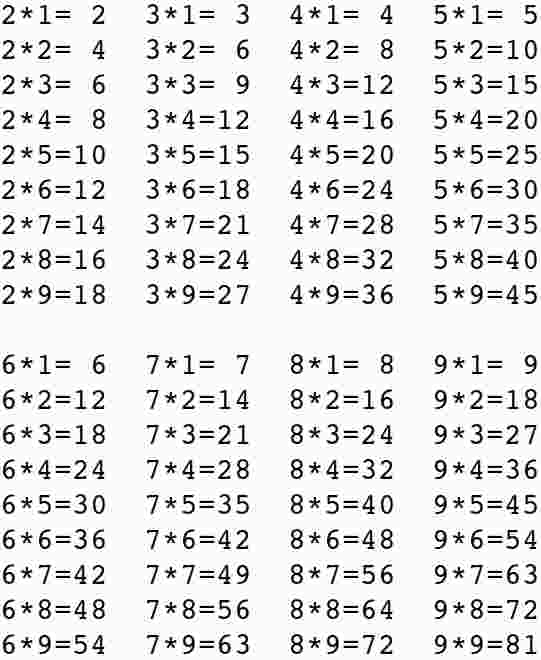
\includegraphics[height=12cm]{../solutions/fig/JA007fig}
\end{figure}

\subsection{解題思惟}
可以想成輸出兩個大群組的九九乘法表,當輸出第r (r=0, 1) 個群組時,
``被乘數"$=j+r\times4.$ (j=2, 3, 4, 5)。
			
\subsection{程式碼}
\begin{cppcode}
#include <cstdio>

int main()
{
	for (int r=0; r<2; r++) { //兩個群組
		for (int i=1; i<=9; i++) { //第i列的乘數是i
			for(int j=2; j<=5; j++) { //被乘數=j+r*4
				printf("%d*%d=%2d  ", j+r*4, i, i*(j+r*4));
			}
			printf("\n");
		}
		printf("\n");
	}
	return 0;
}
\end{cppcode}

\section{河內塔基本題}
依河內塔規則,將環從A移到C,B為輔助。輸入環的個數n,輸出所有移動過程。

\subsection{解題思惟}
本題使用遞迴解題較為容易。假設 hanoi(int n, char from, char to, char buf) 代表可以將n個環,從from移到to,且暫存為buf的函式。當n為1的時候,直接移動即可,
若n>1,則可以先將n-1個環從from移到buf,然後移動第n個環,再將n-1個環從buf移到to,如下:
\begin{inside}
	hanoi(n-1, from, buf, to);
	cout << from << " => " << to << endl;
	hanoi(n-1, buf, to, from);
\end{inside}	
			
\subsection{程式碼}
\begin{cppcode}
#include <iostream>

using namespace std;

void hanoi(int n, char from, char to, char buf);

int main()
{
	int n;
	cin >> n;
	hanoi(n, 'A', 'C', 'B');
	return 0;
}

void hanoi(int n, char from, char to, char buf)
{
	if (n==1) {
		cout << from << " => " << to << endl;
	} else {
		hanoi(n-1, from, buf, to);
		cout << from << " => " << to << endl;
		hanoi(n-1, buf, to, from);
	}
}
\end{cppcode}

\section{印等腰三角形}
輸入N,印出一個N列的等腰三角形,其中第I列有2*I-1個\#,且左右對稱。

\subsection{解題思惟}
\begin{enumerate}
	\item N列的輸出,可以跑一個迴圈,令i等於1到N來處理。
	\item 第N列有2*N-1個\#,且前面沒有空白。
	\item 第N-1列有2*(N-1)-1個\#,且前面有1個空白。
	\item 依次類推,第i列應該是有2*i-1個\#,且前面有N-i個空白。
\end{enumerate}
			
\subsection{程式碼}
\begin{cppcode}
#include <iostream>

using namespace std;

int main()
{
	int n;
	cin >> n;
	cout << "Input = " << n << endl;
	for (int i=1; i<=n; i++) {
		for (int j=0; j<n-i; j++) cout << " ";
		for (int j=0; j<2*i-1; j++) cout << "#";
		cout << endl;
	}
	return 0;
}
\end{cppcode}

\section{A016 - 三數排序}
輸入三個正整數 a、b、c,將 a、b、c 從小排到大並輸出。
\subsection{解題思維}
\begin{enumerate}
\item a,b,c三數排序時,可以先比a和b,如果a>b則交換兩個數,使a<b,之後再比b和c,順序不對就交換,使b<c,此時c為最大值。最後再比較和調整一次a和b即可。
	\begin{inside}
	if (a>b) swap(a, b);
	if (b>c) swap(b, c);
	if (a>b) swap(a, b);
	\end{inside}
\item 交換兩數x和y,在\cc{}中可以直接使用swap函式,如果是在C裡面,則常用的方法是宣告另一個暫存變數t,然後使用以下敘述:
	\begin{inside}
		t=x; x=y; y=t;
	\end{inside}
\item 其實排序有很多種方法,以上的排序法稱為氣泡排序法,它的基本原理是兩兩相比,順序不對就互相交換,這樣依序比過一輪,最大的就跑到最右邊了。之後再比第二輪,可以把次大的送到右邊第二位,依此類推。還不明白的讀者可自行上網查詢,或查看一般程式書籍,以進一步了解其原理和作法。
\end{enumerate}

\subsection{程式碼}
\begin{cppcode}
	#include <iostream>

	using namespace std;
	
	int main()
	{
		int a, b, c;
		cin >> a >> b >> c;
		if (a>b) swap(a, b);
		if (b>c) swap(b, c);
		if (a>b) swap(a, b);
		cout << a << " " << b << " " << c;
		return 0;
	}
\end{cppcode}


\section{A029 - 費式數列}
費氏數列定義如下 $f(0)=0, f(1)=1, f(n)=f(n-1)+f(n-2)$;請從螢幕輸入一個正整數n,輸出$f(n)$。

\subsection{解題思惟}

\begin{enumerate}
\item 本題可以使用遞迴或非遞迴方式求解。先討論遞迴寫法。
\item 遞迴函式f(n),如果n<2,回傳n即可,n>=2時,回傳f(n-1)+f(n-2)即可。
\item 如果不使用遞迴的話,可以設fn, fnm1, fnm2三個變數,分別表示f(n), f(n-1)及f(n-2),先設好f(n-1)及f(n-2)的初始值,然後每次計算fn=fnm1+fnm2,算完後令 fnm2=fnm1, fnm1=fn,不斷重覆即可,重覆次數為n-1次。
\end{enumerate}

\subsection{程式碼}
遞迴版本
\begin{cppcode}
#include <cstdio>

int f(int n);

int main()
{
	int n;
	scanf("%d", &n);
	printf("%d", f(n));
	return 0;
}

int f(int n)
{
	if (n<2) return n;
	return f(n-1)+f(n-2);
}
\end{cppcode}
非遞迴版本
\begin{cppcode}
#include <cstdio>

int main()
{
	int n, fn, fnm1=1, fnm2=0;
	scanf("%d", &n);
	if (n<2) fn=n;
	else for (int i=2; i<=n; i++) {
		fn = fnm1 + fnm2;
		fnm2 = fnm1;
		fnm1 = fn;
	}
	printf("%d", fn);
	return 0;
}
\end{cppcode}

\section{F021 - 奇偶數}
輸入一整數,輸出其奇偶性。

\subsection{解題思維}
判斷整數n是否為奇數的方法,可求其除以2的餘數,若非0即為奇數,或者將其和1做位元\&的運算,如果非0即為奇數。
\begin{inside}
	if (n%2) { // n 為奇數,或者
	if (n&1) { // n 為奇數
\end{inside}	
\subsection{程式碼}
\begin{cppcode}
	#include <iostream>
	
	using namespace std;
	
	int main ()
	{
		int a;
		cin >> a;
		if (a%2) cout << "odd";
		else cout << "even";
		return 0;
	}
\end{cppcode}

\section{G001 - 長寬高算體積}
輸入長方體的長寬高,輸出其體積。
\subsection{解題思惟}
宣告三個變數,取得使用者輸入後,計算其乘積輸出即可。
\subsection{程式碼}
\begin{cppcode}
#include <iostream>

using namespace std;

int main()
{
	int length, width, height;
	cin >> length >> width >> height;
	cout << length * width * height;
	return 0;
}
\end{cppcode}

\section{G004 - 蝸牛爬牆壁}
資訊學院牆壁高 a 公尺,蝸牛從 b 公尺高的地方往上爬,白天可以往上爬 c 公尺,但是晚上睡著了會下降 d 公尺,請問蝸牛幾天後可以爬上屋頂?
\subsection{解題思惟}
\begin{enumerate}
	\item 這一題可以有兩類解法,第一種依題意設立變數a, b, c, d與天數,然後使用迴圈和題目規則去計算所需的天數;第二種則是使用代數的推導去計算所需的天數。
	\item 第一種的作法比較直接,假設有a,b,c,d, 及day=0,可跑以下迴圈計算所需的天數:
	\begin{inside}
		while (b<a) { // 還沒爬到
			day++; b+=c; // 多一天,並且可以爬到高度 b=b+c
			if (b>=a) break; // 已經爬到了,跳出迴圈
			b -= d; // 還沒到的話,晚上會掉下 d 公尺
		}
	\end{inside}
	\item 第二種解法,假設所需天數為x,則x-1天白天可以到達的高度為 b+(c-d)(x-2)+c,這個值應該小於a;而第x天白天可以到達的高度為 b+(c-d)(x-1)+c,這個高度應該大於等於a,故可以得到以下的不等式:
	$$ b+(c-d)(x-2)+c < a \le b+(c-d)(x-1)+c$$
	稍作整理可以得到以下的不等式:
	$$ \frac{a-b-c}{c-d}+1 \le x < \frac{a-b-c}{c-d}+2$$
	換句話說,滿足$x\ge \frac{a-b-c}{c-d}+1$的最小整數$x$就是答案。如果m和n都是整數,要找整數$x\ge\frac{m}{n}$,因為在C/\cc{}語言中,整數除以整數只取整數,所以稍加思考,可以得到最小整數$x=\frac{m+n-1}{n}$(思考一下為什麼?),所以這一題的答案為$x=\frac{a-b-d-1}{c-d}+1$。讀者可以實際驗證看看是否正確。
\end{enumerate}
\subsection{程式碼}
\begin{cppcode}
#include <stdio.h>
int main()
{
	int a, b, c, d, day=0;
	scanf("%d%d%d%d", &a, &b, &c, &d);
	while (b<a) {
		day++; b+=c;
		if (b>=a) break;
		b-=d;
	}
	printf("%d", day);
	return 0;
}
\end{cppcode}

\section{1到100奇數相加}
使用 for 迴圈計算 1+3+5+...+99。

\subsection{解題思惟}
本題是 for 迴圈的基本題。
for迴圈的用法是for(起始值; 條件式; 更新值),本題的for迴圈寫法如下:
\begin{inside}
	for (int i=1; i<=100; i+=2) sum += i;
\end{inside}

\subsection{程式碼}
\begin{cppcode}
#include <iostream>

using namespace std;

int main()
{
	int sum=0;
	for (int i=1; i<=100; i+=2) sum += i;
	cout << sum;
	return 0;
}
\end{cppcode}

\section{取出一個整數的每個位數}
輸入一個整數,把每個位數印出來(從個位數開始印)。輸出時,用換行符號分隔每一個數。

\subsection{解題思惟}
\begin{enumerate}
	\item 取出一個整數n的個位,可以使用n\%10求餘數即可。
	\item 將一個整數n的個位去掉,可以使用 n/=10 求商即可。
	\item 如果 n>0,表示n還有位數可取,可以重覆以上的計算。
\end{enumerate}

\subsection{程式碼}
\begin{cppcode}
#include <iostream>

using namespace std;

int main()
{
	int n;
	cin >> n;
	while (n) {
		cout << n%10 << endl;
		n/=10;
	}
	return 0;
}
\end{cppcode}

\section{M90H011 - 整數商餘}
輸入兩整數m和n,輸出m除以n之商及餘數。
\subsection{解題思惟}
整數相除仍為整數,也就是相除的商;另外求餘數可使用\%運算子。又本題之輸出帶有一點格式,使用printf函式輸出會比較方便一點。
\subsection{程式碼}
\begin{cppcode}
#include <cstdio>

int main()
{
	int m, n;
	scanf("%d%d", &m, &n); 
	printf("\n%d / %d=%d", m, n, m / n);
	printf("\n%d mod %d=%d", m, n, m % n);
	return 0;
}
\end{cppcode}



\end{document}
